The working paper used the algorithm on 2 cases.
\begin{enumerate}
    \item Regular land space
    \begin{enumerate}
        \item Single Wind Speed, Multiple Wind Direction
        \item Multiple Wind Speed, Multiple Wind Direction
    \end{enumerate}
    \item Irregular Land Space
    \begin{enumerate}
        \item Multiple Wind Speed, Multiple Wind Direction
    \end{enumerate}
\end{enumerate}

    The Phase I of the algorithm is tested on four different population sizes, 100, 200, 300, 400 and 500 to observe the behavior of the algorithm and the solution for different population sizes. Other parameters used for the Phase I of the algorithm is shown in Table \ref{paramPhaseI}. Moreover, the wind turbine used for the problem was the same as with the previous examples (see Table \ref{specsA} for specifications).
    
    \begin{table}[H]
        \centering
        \begin{tabular}{|c|c|} \hline
            Maximum Generation & 1000 \\ \hline
            Crossover rate & 70\% \\ \hline
            Mutation Rate & 2\% \\ \hline
        \end{tabular}
        \caption{Controlling parameters for the Phase I of the algorithm}
        \label{paramPhaseI}
    \end{table}
    
    \begin{table}[H]
        \centering
        \begin{tabular}{|c|c|} \hline
            Hub Height $z$ & 60m \\ \hline
            Rotor Radius $r_o$ & 20m \\ \hline
            Thrust Coefficient $C_T$ & 0.88 \\ \hline
            Ground Roughness $z_o$ & 0.3m \\ \hline
            Axial Induction Factor $a$ & 0.3267949 \\ \hline
            Entrainment Constant $\beta$ & 0.09437 \\ \hline
            Downstream Radius $r_1$ & 27.881m \\ \hline
        \end{tabular}
        \caption{Specifications of the Wind Turbine Used for the Problem.}
        \label{specsA}
    \end{table}
    
    \subsection{Regular Land Space}
    For the regular land space, the space used has a size of 2km by 2km, dividing the matrix model into 10 rows and 10 columns where each cell in the matrix has a size of 200 meters by 200 meters. A wind turbine can be located only at the center of a cell and only one wind turbine can occupy a cell in the matrix. For the the first case, the is only a single constant wind speed for the whole year, 12 meters per second and exists in all wind directions with equal fraction of occurrences.
    
    The goal of the problem is to find the optimal number of wind turbines by maximizing the power output while minimizing the cost. Assuming that the optimal number of wind turbines $N$ lies between 10 and 50 (inclusive), and assuming the the computer needs 1 microsecond to compute the fitness of a single configuration and compare it with other configurations, going through all possible configurations would take $2.17x10^{16}$ years to finish, which is why a heuristics method is used.
    
    The algorithm was written in Java and executed on a portable laptop AMD Ryzen 5 2500U processor and 4 GB RAM. The result of the Phase I of the algorithm is shown in Table \ref{resultsCaseA}.
    
    \singlespacing
    \begin{table}[H]
        \centering
        \begin{tabular}{|c|c|c|c|c|c|} \hline
            \textbf{} & \multicolumn{5}{c|}{\textbf{Population Size}} \\ \hline
No. of Turbines     & 100     & 200     & 300     & 400    & 500    \\ \hline
10	 & 	0.001855001	 & 	0.001852028	 & 	0.001849942	 & 	0.001851119	 & 	0.001849942	 \\ \hline
11	 & 	0.001844735	 & 	0.001844231	 & 	0.001843478	 & 	0.001844373	 & 	0.00185211	 \\ \hline
12	 & 	0.001835448	 & 	0.001835268	 & 	0.001834293	 & 	0.001833353	 & 	0.00183353	 \\ \hline
13	 & 	0.001826519	 & 	0.001823489	 & 	0.001824564	 & 	0.001823207	 & 	0.001823207	 \\ \hline
14	 & 	0.001812275	 & 	0.001811836	 & 	0.001811836	 & 	0.001811801	 & 	0.001811836	 \\ \hline
15	 & 	0.001801313	 & 	0.001799587	 & 	0.001798592	 & 	0.001798592	 & 	0.001798592	 \\ \hline
16	 & 	0.00178496	 & 	0.001786322	 & 	0.001784734	 & 	0.001784734	 & 	0.001784734	 \\ \hline
17	 & 	0.00177102	 & 	0.001770966	 & 	0.00177102	 & 	0.0017712	 & 	0.001770866	 \\ \hline
18	 & 	0.001756775	 & 	0.001756116	 & 	0.001755951	 & 	0.001755951	 & 	0.001755391	 \\ \hline
19	 & 	0.001741812	 & 	0.001740865	 & 	0.001740038	 & 	0.001739877	 & 	0.001740084	 \\ \hline
20	 & 	0.001723638	 & 	0.001723769	 & 	0.001723769	 & 	0.001723639	 & 	0.001723366	 \\ \hline
21	 & 	0.001709319	 & 	0.001706456	 & 	0.00170848	 & 	0.001706456	 & 	0.001706456	 \\ \hline
22	 & 	0.001691424	 & 	0.001691861	 & 	0.001689401	 & 	0.001689401	 & 	0.001692148	 \\ \hline
23	 & 	0.001676473	 & 	0.001675649	 & 	0.001675684	 & 	0.0016756	 & 	0.0016756	 \\ \hline
24	 & 	0.00166233	 & 	0.00166024	 & 	0.001660524	 & 	0.00166024	 & 	0.00166024	 \\ \hline
25	 & 	0.001646532	 & 	0.001646008	 & 	0.001645911	 & 	0.001645911	 & 	0.001645849	 \\ \hline
26	 & 	0.001633758	 & 	0.001631942	 & 	0.001632194	 & 	0.001632215	 & 	0.001632194	 \\ \hline
27	 & 	0.001619477	 & 	0.001619417	 & 	0.00161926	 & 	0.001619417	 & 	0.001619477	 \\ \hline
28	 & 	0.001608929	 & 	0.001607189	 & 	0.001607189	 & 	0.001607189	 & 	0.001607326	 \\ \hline
29	 & 	0.001597295	 & 	0.001597263	 & 	0.001597263	 & 	0.001597263	 & 	0.001597263	 \\ \hline
30	 & 	0.001587876	 & 	0.001587876	 & 	0.001587826	 & 	0.001587876	 & 	0.001587826	 \\ \hline
31	 & 	0.001579261	 & 	0.001579245	 & 	0.001579245	 & 	0.001579245	 & 	0.001579245	 \\ \hline
32	 & 	0.001571261	 & 	0.001571238	 & 	0.001571238	 & 	0.001571238	 & 	0.001571238	 \\ \hline
33	 & 	0.001565627	 & 	0.001565627	 & 	0.001565627	 & 	0.001565627	 & 	0.001576526	 \\ \hline
34	 & 	0.001561213	 & 	0.001561213	 & 	0.001561213	 & 	0.001561213	 & 	0.001561213	 \\ \hline
35	 & 	0.001558506	 & 	0.001557478	 & 	0.001557478	 & 	0.001557478	 & 	0.001557478	 \\ \hline
36	 & 	0.001554488	 & 	0.001554316	 & 	0.001554316	 & 	0.001554316	 & 	0.001554316	 \\ \hline
37	 & 	0.001552811	 & 	0.001552811	 & 	0.001552811	 & 	0.001552811	 & 	0.001552811	 \\ \hline
38	 & 	0.001552458	 & 	0.001552458	 & 	0.001552458	 & 	0.001552458	 & 	0.001552458	 \\ \hline
39	 & 	0.00155298	 & 	0.001552427	 & 	0.001552427	 & 	0.001552427	 & 	0.001552427	 \\ \hline
40	 & 	0.001555158	 & 	0.001554994	 & 	0.001554994	 & 	0.001555158	 & 	0.001565826	 \\ \hline
41	 & 	0.001558535	 & 	0.00155835	 & 	0.00155835	 & 	0.00155835	 & 	0.001558535	 \\ \hline
42	 & 	0.001563578	 & 	0.001562644	 & 	0.001562644	 & 	0.001562644	 & 	0.001562613	 \\ \hline
43	 & 	0.001571681	 & 	0.001567161	 & 	0.001567161	 & 	0.001567161	 & 	0.001567161	 \\ \hline
44	 & 	0.001573073	 & 	0.00157404	 & 	0.001572219	 & 	0.001572219	 & 	0.001572219	 \\ \hline
45	 & 	0.001580809	 & 	0.001580203	 & 	0.001578525	 & 	0.001578525	 & 	0.001578525	 \\ \hline
46	 & 	0.001584929	 & 	0.001584929	 & 	0.001584929	 & 	0.001584929	 & 	0.001584929	 \\ \hline
47	 & 	0.001597062	 & 	0.001591947	 & 	0.001591947	 & 	0.001591947	 & 	0.001591947	 \\ \hline
48	 & 	0.001603242	 & 	0.001600855	 & 	0.001599005	 & 	0.001599005	 & 	0.001601037	 \\ \hline
49	 & 	0.001609715	 & 	0.00160787	 & 	0.00160787	 & 	0.00160787	 & 	0.00160787	 \\ \hline
50	 & 	0.00162134	 & 	0.001618372	 & 	0.001618324	 & 	0.001616722	 & 	0.001618556	 \\ \hline
        \end{tabular}
        \caption{Fitness of each population Size for different number of wind turbines without the Local Search Algorithm}
        \label{resultsCaseA}
    \end{table}
    \doublespacing
    
    From Table \ref{resultsCaseA}, the following are observed.
    \begin{enumerate}
        \item A population size of 100 was not enough to (almost) reach the optimal solution. There were never a case the population size of 100 alone gave the best solution.
        \item A bigger population size does not guarantee that the algorithm will give a better solution. There were cases that:
        \begin{enumerate}
            \item A population size of 200 alone gave the best solution among the other population size at $N=26$.
            \item A population size of 300 alone gave the best solution among the other population size at $N=11$ and $N=27$.
            \item A population size of 400 alone gave the best solution among the other population size at $N=12$, $N=14$, $N=19$ and $N=11$.
            \item A population size of 500 alone gave the best solution among the other population size at $N=17$, $N=18$, $N=20$, $N=37$ and $N=42$.
        \end{enumerate}
    \end{enumerate}
    \singlespacing
    \begin{table}[H]
        \centering
        \begin{tabular}{|c|c|c|c|c|c|} \hline
            \textbf{} & \multicolumn{5}{c|}{\textbf{Population Size}} \\ \hline
                      & 100     & 200     & 300     & 400    & 500    \\ \hline
           10	 & 	0.001849942	 & 	0.001849942	 & 	0.001849942	 & 	0.001849942	 & 	0.001849942	 \\ \hline
11	 & 	0.001844363	 & 	0.001844231	 & 	0.001843478	 & 	0.001844373	 & 	0.001843478	 \\ \hline
12	 & 	0.00183353	 & 	0.001834173	 & 	0.001834293	 & 	0.001833353	 & 	0.00183353	 \\ \hline
13	 & 	0.001823207	 & 	0.001823207	 & 	0.001823207	 & 	0.001823207	 & 	0.001823207	 \\ \hline
14	 & 	0.001812275	 & 	0.001811836	 & 	0.001811836	 & 	0.001811801	 & 	0.001811836	 \\ \hline
15	 & 	0.001799258	 & 	0.001798592	 & 	0.001798592	 & 	0.001798592	 & 	0.001798592	 \\ \hline
16	 & 	0.001783735	 & 	0.001783735	 & 	0.001784734	 & 	0.001784734	 & 	0.001784734	 \\ \hline
17	 & 	0.00177102	 & 	0.001770295	 & 	0.00177102	 & 	0.0017712	 & 	0.001770866	 \\ \hline
18	 & 	0.001755391	 & 	0.001755923	 & 	0.001755951	 & 	0.001755951	 & 	0.001755391	 \\ \hline
19	 & 	0.001740714	 & 	0.001740865	 & 	0.001740038	 & 	0.001739877	 & 	0.001740084	 \\ \hline
20	 & 	0.001723609	 & 	0.001723639	 & 	0.001723639	 & 	0.001723639	 & 	0.001723366	 \\ \hline
21	 & 	0.001708368	 & 	0.001706456	 & 	0.00170848	 & 	0.001706456	 & 	0.001706456	 \\ \hline
22	 & 	0.001691267	 & 	0.001691861	 & 	0.001689401	 & 	0.001689401	 & 	0.001692148	 \\ \hline
23	 & 	0.00167591	 & 	0.0016756	 & 	0.00167407	 & 	0.0016756	 & 	0.0016756	 \\ \hline
24	 & 	0.001660524	 & 	0.00166024	 & 	0.001660524	 & 	0.00166024	 & 	0.00166024	 \\ \hline
25	 & 	0.001646008	 & 	0.001646008	 & 	0.001645911	 & 	0.001645911	 & 	0.001645849	 \\ \hline
26	 & 	0.001631942	 & 	0.001631942	 & 	0.001632194	 & 	0.001632215	 & 	0.001632194	 \\ \hline
27	 & 	0.001619477	 & 	0.001619417	 & 	0.00161926	 & 	0.001619417	 & 	0.001619477	 \\ \hline
28	 & 	0.001607497	 & 	0.001607189	 & 	0.001607189	 & 	0.001607189	 & 	0.001607326	 \\ \hline
29	 & 	0.001597295	 & 	0.001597263	 & 	0.001597263	 & 	0.001597263	 & 	0.001597263	 \\ \hline
30	 & 	0.001587826	 & 	0.001587826	 & 	0.001587826	 & 	0.001587826	 & 	0.001587826	 \\ \hline
31	 & 	0.001579245	 & 	0.001579245	 & 	0.001579245	 & 	0.001579245	 & 	0.001579245	 \\ \hline
32	 & 	0.001571261	 & 	0.001571238	 & 	0.001571238	 & 	0.001571238	 & 	0.001571238	 \\ \hline
33	 & 	0.001565627	 & 	0.001565627	 & 	0.001565627	 & 	0.001565627	 & 	0.001565627	 \\ \hline
34	 & 	0.001561213	 & 	0.001561213	 & 	0.001561213	 & 	0.001561213	 & 	0.001561213	 \\ \hline
35	 & 	0.001557478	 & 	0.001557478	 & 	0.001557478	 & 	0.001557478	 & 	0.001557478	 \\ \hline
36	 & 	0.001554316	 & 	0.001554316	 & 	0.001554316	 & 	0.001554316	 & 	0.001554316	 \\ \hline
37	 & 	0.001552811	 & 	0.001552811	 & 	0.001552811	 & 	0.001552811	 & 	0.001552811	 \\ \hline
38	 & 	0.001552458	 & 	0.001552458	 & 	0.001552458	 & 	0.001552458	 & 	0.001552458	 \\ \hline
39	 & 	0.001552427	 & 	0.001552427	 & 	0.001552427	 & 	0.001552427	 & 	0.001552427	 \\ \hline
40	 & 	0.001555158	 & 	0.001554994	 & 	0.001554994	 & 	0.001555158	 & 	0.001555158	 \\ \hline
41	 & 	0.001558535	 & 	0.00155835	 & 	0.00155835	 & 	0.00155835	 & 	0.001558535	 \\ \hline
42	 & 	0.001562644	 & 	0.001562644	 & 	0.001562644	 & 	0.001562644	 & 	0.001562613	 \\ \hline
43	 & 	0.001568304	 & 	0.001567161	 & 	0.001567161	 & 	0.001567161	 & 	0.001567161	 \\ \hline
44	 & 	0.001572219	 & 	0.00157404	 & 	0.001572219	 & 	0.001572219	 & 	0.001572219	 \\ \hline
45	 & 	0.001580809	 & 	0.001578525	 & 	0.001578525	 & 	0.001578525	 & 	0.001578525	 \\ \hline
46	 & 	0.001584929	 & 	0.001584929	 & 	0.001584929	 & 	0.001584929	 & 	0.001584929	 \\ \hline
47	 & 	0.001594359	 & 	0.001591947	 & 	0.001591947	 & 	0.001591947	 & 	0.001591947	 \\ \hline
48	 & 	0.001599005	 & 	0.001599005	 & 	0.001599005	 & 	0.001599005	 & 	0.001601037	 \\ \hline
49	 & 	0.00160787	 & 	0.00160787	 & 	0.00160787	 & 	0.00160787	 & 	0.00160787	 \\ \hline
50	 & 	0.00162134	 & 	0.001616722	 & 	0.001616722	 & 	0.001616722	 & 	0.001618556	 \\ \hline

        \end{tabular}
        \caption{Fitness of each population Size for different number of turbines with the Local Search Algorithm}
        \label{resultsCaseA2}
    \end{table}
    \doublespacing
    
    %SHOW THE PLOT OF THE RESULTS OF THE GA AND THE LOCAL SEARCH SA IISANG GRAPH PARA MA COMPARE SILA DALAWA
    \begin{figure}[H]
        \centering
        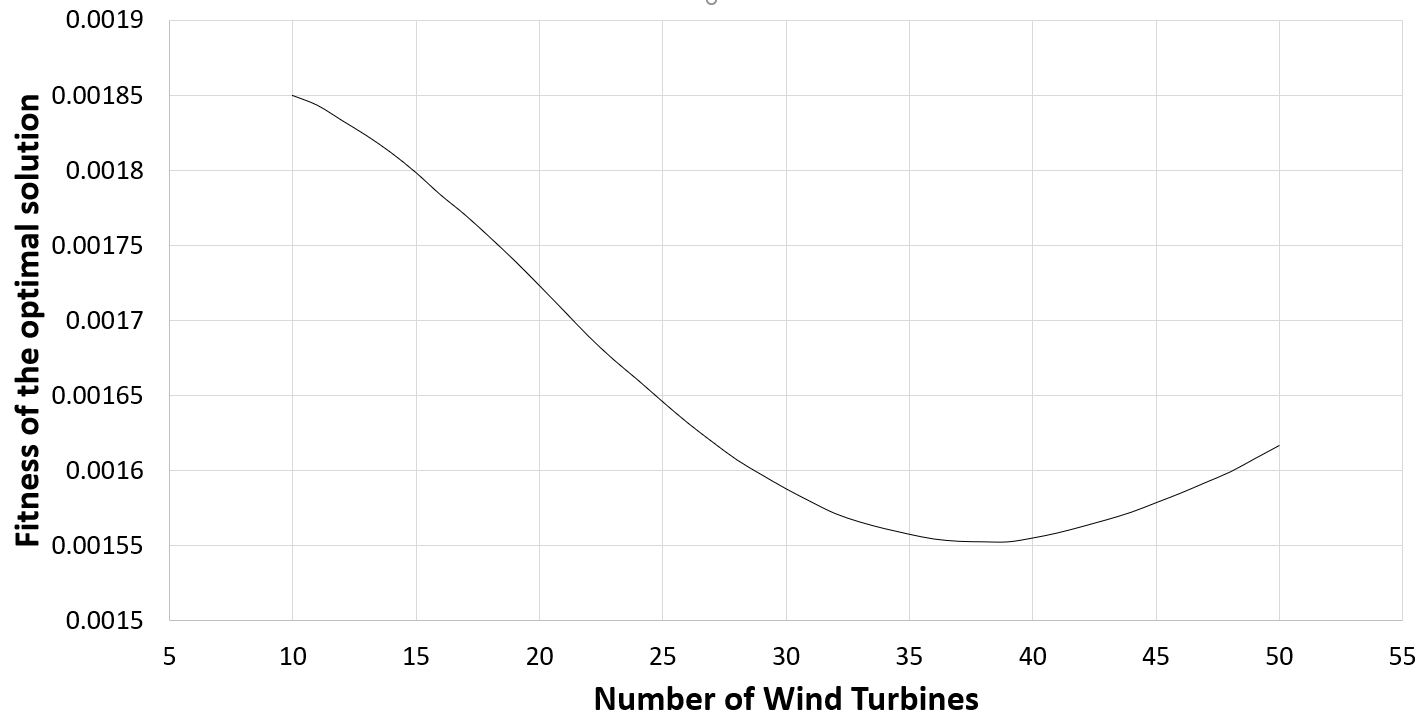
\includegraphics[width=\textwidth]{Figures/graphA.png}
        \caption{Optimum objective Vs number of turbines obtained from BRCGA+LS for the case of single speed multiple directions, (2 km$\cdot$2 km land space)}
        \label{graphA}
    \end{figure}
    
    %EXPLAIN HOW THE POPULATION SIZE AFFECTS THE NEED FRO LOCAL SEARCH
    Without the use of Local Search Algorithm, the population size greatly influences the fitness of the experiment. Evidently, if the difference in the population size shows that the higher the population size the better the fitness. For example in table \ref{resultsCaseA} at $10$ turbines, the initial fitness in each population size greatly varies with fully optimized fitness at $300$ and $500$ and worse fitness at $100$. Looking at the table \ref{resultsCaseA2}, the fitness in each population at the same number of turbines at $10$ is all identical and fully optimized. The results also shows that the fitness in each population is better at higher population without the use of Local Search Algorithm at table \ref{resultsCaseA}. Note that this difference in fitness means that the population size must be high enough to yield better results but not too much high to avoid too much variability for the solution set.
    
    %TELL THE OPTIMAL SOLUTION, THAT IS N=39
    The optimal solution for the experiment as shown in the table \ref{resultsCaseA2} is at $N = 39$ with the fitness of $0.001552427$. This means that at $39$ turbines, there are enough wind turbines to supply the maximum power output and minimizing wake interaction in the wind farm. The optimal configuration of 39 wind turbines on a 2km by 2km wind farm with single wind speed and multiple wind direction is shown in Figure \ref{optimalA}.

    %SHOW THE IMAGE OF THE OPTIMAL SOLUTION FOR N=39
    \begin{figure}[H]
        \centering
        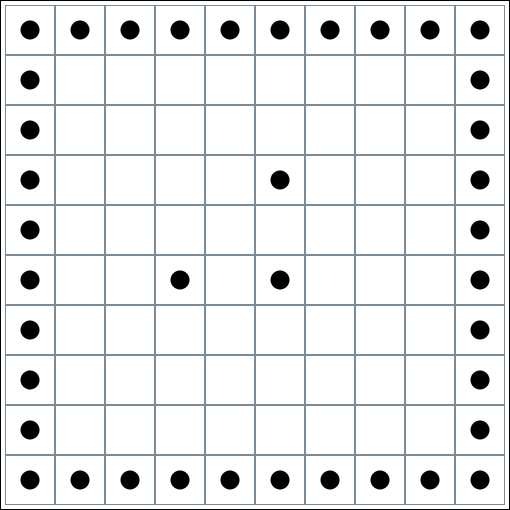
\includegraphics[width=15cm]{Figures/optimalA.png}
        \caption{Optimal Configuration of 39 Wind Turbines on a 2km by 2km Wind Farm with a constant wind speed of 12 meters per second blowing in all directions with equal fraction of occurrences throughout the year.}
        \label{optimalA}
    \end{figure}
    
    %SHOW THE COMPUTATION OF POWER, COST THEN FITNESS.
    %STEPS:
    %FOR EVERY WIND DIRECTION
    %   FOR EVERY WIND TURBINE
    %       FOR EVERY UPSTREAM WIND TURBINE
    %           COMPUTE WIND_SPEED_DUE_TO_UPSTREAM
    %           COMPUTE POWER AND ADD IT TO THE TOTAL POWER
    %COMPUTE COST
    %COMPUTE FITNESS
    
    %THIS MARKS THE START OF THE RESULTS OF CASE 1B (REGULAR LAND SPACE, MULT WIND SPEED, MULT WIND DIRECTION
    
    For the second case, the working paper used the algorithm to find the optimal number of wind turbines on a 10km by 10km wind farm where the wind blows at different velocities (different speed and direction) with different fraction of occurrences, where the optimal number of wind turbines is assumed to be between 10 and 50 (inclusive). The fraction of occurrences for every pair of wind speed and wind direction are shown in Table \ref{fracOfOccur}.
    \begin{table}[h]
        \centering
        \begin{tabular}{|c|c|} \hline
             &  \\ \hline
            \textbf{8 m/s} &  \\ \hline
            \textbf{12 m/s} &  \\ \hline
            \textbf{17 m/s} &  \\ \hline
        \end{tabular}
        \caption{Fraction of occurrences for every pair of wind speed and wind direction for the case of different wind speed and different wind direction.}
        \label{fracOfOccur}
    \end{table}
    
    %TABLE - RESULT OF GA
    %TABLE - RESULT OF GA+LS
    %GRAPH - FITNESS VS NUMBER OF WID=ND TURBINES
    
    0 - 180
    10 - 190
    20 - 200
    30 - 210
    ...
    90 - 270
    ...
    180 - 0
    ...
    270 - 90
    ...
    350 - 170
    
    \subsection{Irregular Land Space}
    The algorithm was also used on an irregular land space to show that it still works with irregularly shaped land space. For this case, multiple speed and multiple direction is also used 
    
    
    
    